\documentclass{standalone}
\usepackage{pgfplots}
\pgfplotsset{compat=newest}
\usepgfplotslibrary{patchplots}
\begin{document}
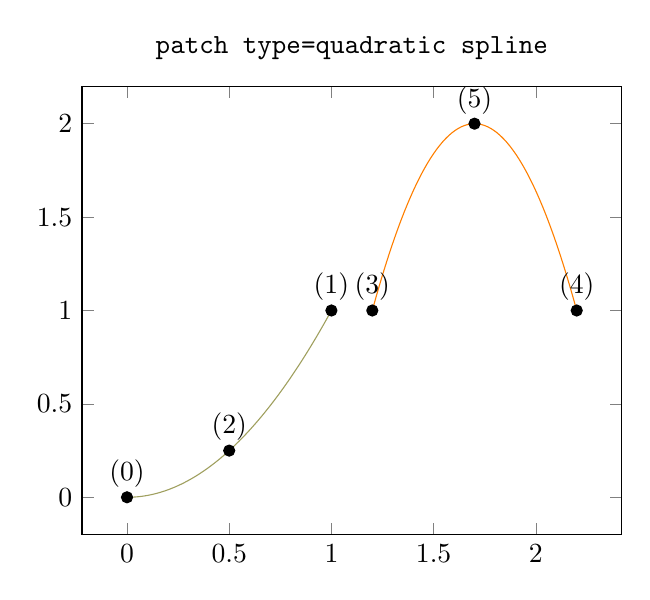
\begin{tikzpicture}
\begin{axis}[nodes near coords={(\coordindex)},
	title={\texttt{patch type=quadratic spline}}]
\addplot[
	mark=*,
	patch,mesh,% without mesh, pgfplots tries to fill
	patch type=quadratic spline]
coordinates {
	% left, right, middle-> first segment
	(0,0) (1,1) (0.5,0.5^2)
	% left, right, middle-> second segment
	(1.2,1) (2.2,1) (1.7,2)
};
\end{axis}
\end{tikzpicture}
\end{document}
